\chapter{Client Software}

With the communication protocol clearly defined in chapters~\ref{sec:tinyframe} and~\ref{sec:units-overview}, respective~\ref{sec:wireless} for the wireless gateway, the implementation of a client software is relatively straightforward. Two proof-of-concept client libraries have been developed, in languages C and Python.

\section{General Library Structure}

The structure of a GEX support library is in all cases similar:

\begin{itemize}
	\item \textbf{USB or serial port access}

		This is the only platform-dependent part of the library. Unix-based systems provide a standardized POSIX API to configure the serial port. A raw access to \gls{USB} endpoints is possible using the libUSB C library. Access to the serial port or \gls{USB} from C on MS Windows has not been investigated, but should be possible using proprietary APIs.

		Accessing the serial port or \gls{USB} endpoints from Python is more straightforward thanks to the cross platform libraries \textit{PySerial} and \textit{PyUSB}.

	\item \textbf{TinyFrame}

		The \textit{TinyFrame} protocol library can be used directly in desktop C applications, and it has been ported to Python and other languages.

	\item \textbf{Higher-level GEX logic}

		The host side of the communication protocol described in chapter~\ref{sec:tinyframe} should be implemented as a part of the library. This includes the reading and writing of configuration files, unit list read-out, command payload building, and asynchronous event parsing.

		Additional utilities may be defined on top of this basic protocol support for the command API of different GEX units, as described in~\ref{sec:units-overview}. Those unit-specific ``drivers'' are available in the provided Python library.
\end{itemize}

\section{Python Library}

The Python GEX library it implements both serial port and raw USB endpoint access, and includes support classes for each unit type. Its development has been proritized over the C library because of its potential to integrate with MATLAB, and the general ease-of-use that comes with the Python syntax.

The library is composed of a \textit{transport}, the core class called \textit{client}, and unit classes. Three transport implementations have been developed; the gateway is accessed by wrapping either of the transports in an instance of \mono{DongleAdapter}.

\begin{itemize}
	\item \mono{TrxSerialSync} -- virtual serial port access with polling for a response

	\item \mono{TrxSerialThread} -- virtual serial port access with a polling thread and semaphore-based notifications

	\item \mono{TrxRawUSB} -- similar to \mono{TrxSerialThread}, but using a raw USB endpoint access
\end{itemize}

The unit classes wrap the command and event \gls{API} described in chapter~\ref{sec:units-overview}; all classes and methods are annotated by documentation comments for easy understanding.

An example Python program showing a pattern with the \gls{LED} matrix driver IS31FL3730 is presented below as an illustration of the library usage. A photo of the produced pattern can be seen in figure~\ref{fig:pydemo}.

\todo[inline]{add left line next to this listing}
\begin{minted}{python}
#!/bin/env python3
import gex
with gex.Client(gex.TrxRawUSB()) as client:
    bus = gex.I2C(client, 'i2c')
    addr = 0x61
    bus.write_reg(addr, 0x00, 0b00011000) # dual matrix
    bus.write_reg(addr, 0x0D, 0b00001110) # 34 mA
    bus.write_reg(addr, 0x19, 64) # set brightness
    # matrix 1
    bus.write_reg(addr, 0x01, [
        0xAA, 0x55, 0xAA, 0x55,
        0xAA, 0x55, 0xAA, 0x55
    ])
    # matrix 2
    bus.write_reg(addr, 0x0E, [
        0xFF, 0x00, 0xFF, 0x00,
        0xFF, 0x00, 0xFF, 0x00
    ])
    # update display
    bus.write_reg(addr, 0x0C, 0x01)
\end{minted}

\begin{figure}[h]
	\centering
	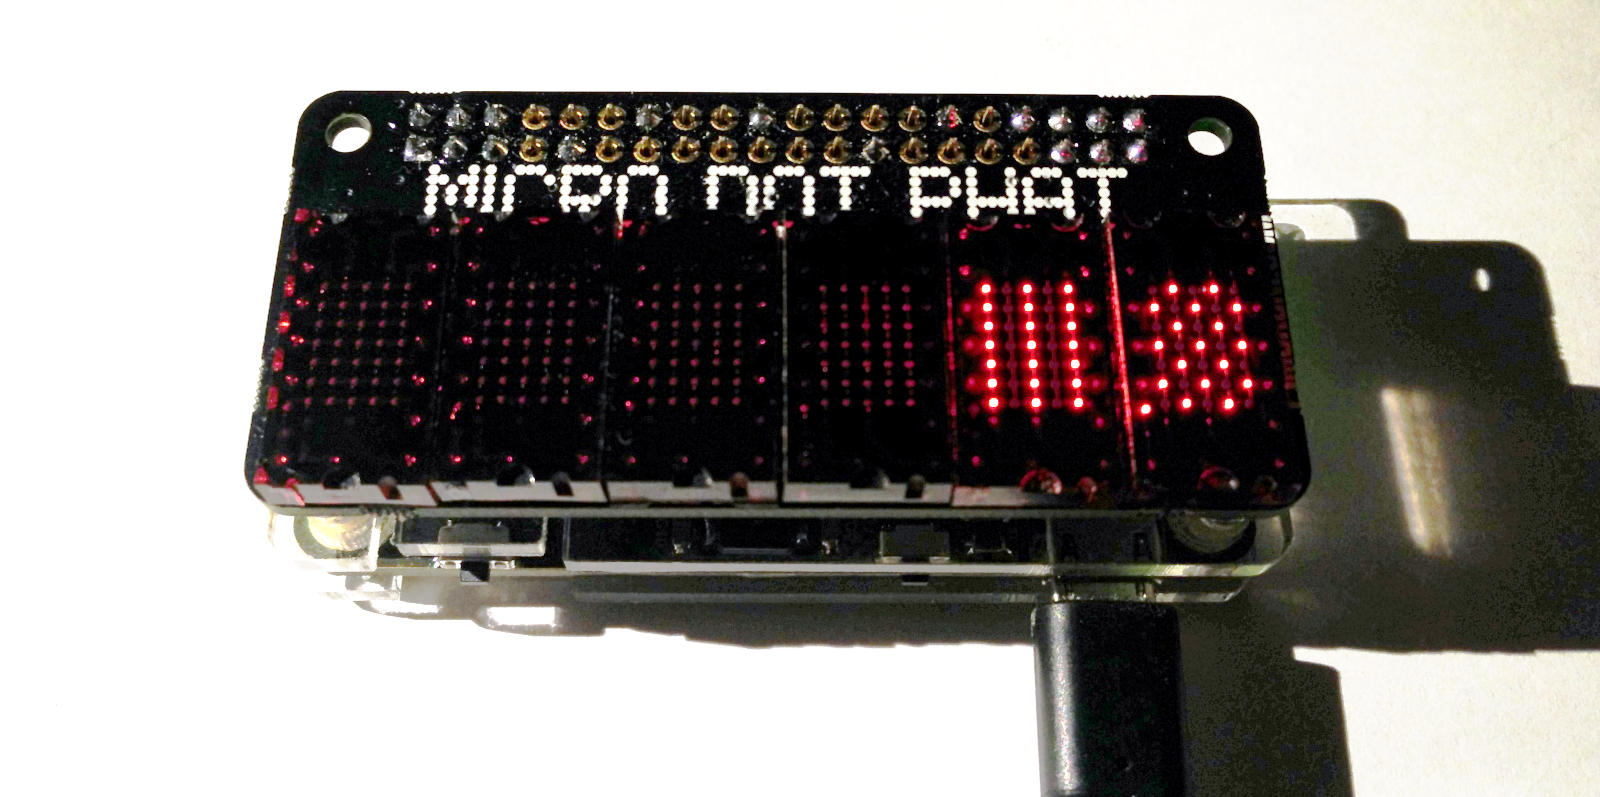
\includegraphics[width=.7\textwidth] {img/phatmtx.jpg}
	\caption{\label{fig:pydemo}GEX Zero with the Micro Dot pHAT add-on board showing a test pattern}
\end{figure}

\section{MATLAB integration}

The Python library can be accessed from MATLAB scripts thanks to the MATLAB's two-way Python integration~\cite{matlabpy}. Controlling GEX from MATLAB may be useful when additional processing is required, e.g. with data from the \gls{ADC}; however, in many cases, an open source alternative native to Python exists that could be used for the same purpose, such as the NumPy and SciPy libraries~\cite{numpyscipy}.

\todo[inline]{add a matlab example}

\section{C Library}

The C library is more simplistic than the Python one; it supports only the serial port transport (\gls{UART} or \gls{CDCACM}) and does not implement asynchronous polling or the unit support drivers. What \textit{is} implement---the transport, a basic protocol handler, and payload building and parsing utilities---is sufficient for most applications, though less convenient than the Python library.

This low-level library is intended for applications where the performance of the Python implementation is insufficient, or where an integration with existing C code is required. The full \gls{API} can be found in the library header files. A C version of the example Python script controlling a \gls{LED} matrix driver follows:

\todo[inline]{add the example}


\todo[inline]{Measurement / evaluation examples here...}





